\chapter{DESARROLLO DEL TRABAJO}
Es el punto en el que se detalla en forma resumida la teoría y práctica del tema sobre el cual se está realizando el trabajo de manera que los conceptos principales queden claros para el estudiante.

\section{Antecedentes}
Para conocer cómo ha ido evolucionando la Información, las Tecnologías de Información y Comunicación, y las Teorías sobre Gestión de la Información, se presentan a continuación los eventos m\'as importantes ocurridos a largo de nuestra historia a partir del año 500 después de Cristo

\begin{enumerate}
\item Priemr Antecedente
\item Segundo Antecedente
\end{enumerate}

\section{Estado del Arte}
Se entiende por Información al conjunto de datos que han sido procesados con la finalidad de establecer un mensaje y generar conocimiento del sistema que lo reciba. El dato es su unidad mínima, el cual por sí solo no posee ningún valor, pero en conjunto genera información. Esta información al ser organizada adecuadamente se convierte en conocimiento y luego del resultado de su análisis se convierte en finalmente sabiduría. \citeA{Blanco2013}

\subsection{Estrategias de Respaldo}

\begin{equation}
f(x)= \left\{ \begin{array}{l||c|l}
x^2 & \mbox{ si } & x<0 \\ \hline
& & \\
x-1 & \mbox{ si } & x>0
\end{array}
\right.	
\end{equation}

\begin{table}[ht]
\centering{
    \fontfamily{ptm}
        \selectfont{
            \rowcolors{1}{gray}{cyan}
            \begin{tabular}{ll}
                $x_{n+1}$ & $|x_{n+1}-x_n|$\\ \hline
                1.20499955540054 & 0.295000445\\
                1.17678931926590 & 0.028210236\\
                1.17650196994274 & 0.000287349\\
                1.17650193990183 & 3.004$\times10^{-8}$\\
                1.17650193990183 & 4.440$\times10^{-16}$\\ \hline
            \end{tabular}
}}
\caption{Iteracion de Newton para $x^2-\cos(x)-1=0$ con $x_0=1.5$}
\end{table}


Este un ejemplo de imagen

\begin{figure}[ht]
\centering
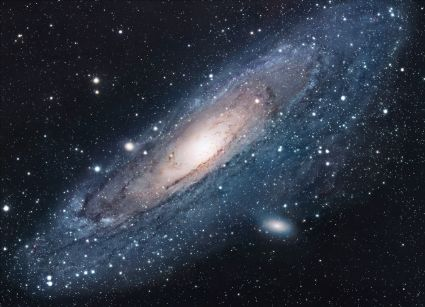
\includegraphics[scale=1.7]{images/universe.jpg}
\caption{The Universe}
\label{fig:universe}
\end{figure}

Terminamos

\subsection{Estrategias de Recuperaci\'on}

\begin{table}[ht]
\centering{
    \fontfamily{ptm}
        \selectfont{
            %\rowcolors{1}{gray}{cyan}
            \begin{tabular}{ll}
                Actividad & Duraci\'on\\ \hline
                Elaboración de los Aspectos Generales del Trabajo de Investigaci\'on   &   10 d\'ias\\
                Elaboración del Marco Te\'orico   &   35 d\'ias\\
                Elaboración del Marco Metodol\'ogico   &   15 d\'ias\\
                Elaboración del Marco Metodol\'ogico   &   15 d\'ias\\
                1.17650193990183 & 4.440$\times10^{-16}$\\ \hline
            \end{tabular}
}}
\caption{Cronograma}
\end{table}